% !TEX root = ../../main.tex

\subsection{Vapour adsorption}

The effects of shaping with \(\rho\)-alumina are 
so far more subtle than the changes encountered when using 
\gls{PVA}, as shown in the corresponding 
study~\cite{chanutObservingEffectsShaping2016}.
As such the characterisation was extended using adsorption
of vapours at room temperature.
The influence of the binder on hydrophobic character of the
material may be of interest for tuning the properties of the 
beads. Here, water and methanol
can serve as probes for small changes in surface properties.
To this end, the same \gls{PVA} samples which were 
used in the previous study were investigated alongside 
the \gls{MRA}-shaped \gls{MOF}.

Due to its surface charges, alumina is a 
hydrophilic substance, with a contact 
angle of \SI{10}{\degree}. It is expected that its 
addition may therefore increase the affinity 
of the resulting pellet towards water. On the other hand,
the \gls{PVA} binder is more hydrophobic, with a water contact
angle of \SI{51}{\degree}. The medium affinity for water
is due to the surface hydroxyl functionalisations, which
can lead to hydrogen bonding.

\begin{figure}[p!]
    \centering
    
    \begin{subfigure}{\linewidth}
        \centering
        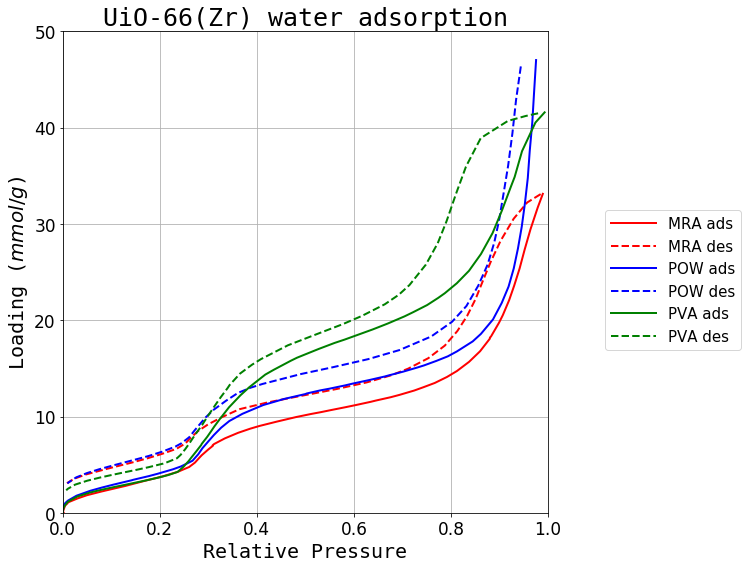
\includegraphics[width=0.45\textwidth]{water/UiO-66(Zr)-water}%
        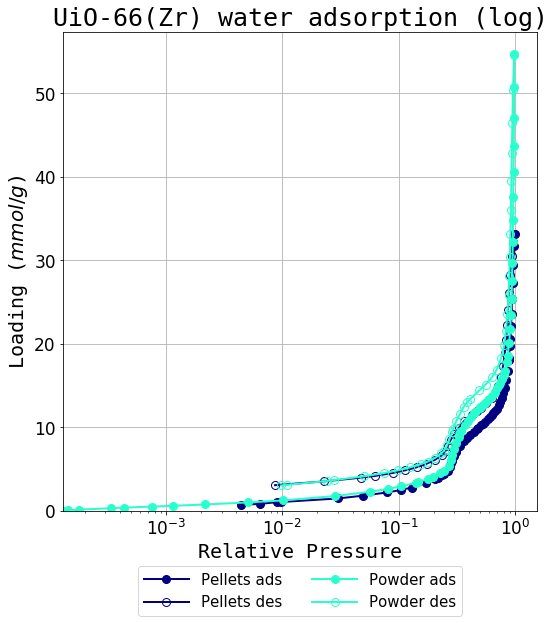
\includegraphics[width=0.45\textwidth]{water/UiO-66(Zr)-water-log}%
        \caption{}\label{shaping:fig:wateruio66}
    \end{subfigure}%

    \begin{subfigure}{\linewidth}
        \centering
        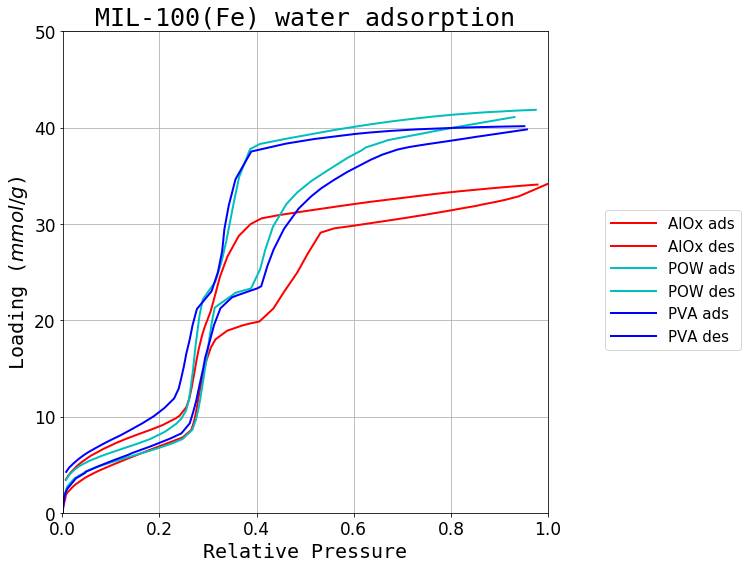
\includegraphics[width=0.45\textwidth]{water/MIL-100(Fe)-water}%
        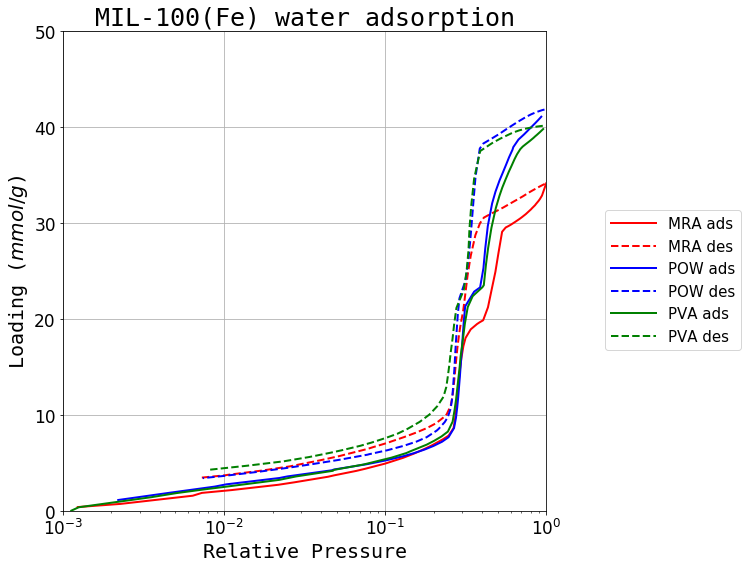
\includegraphics[width=0.45\textwidth]{water/MIL-100(Fe)-water-log}%
        \caption{}\label{shaping:fig:watermil100}
    \end{subfigure}%

    \begin{subfigure}{\linewidth}
        \centering
        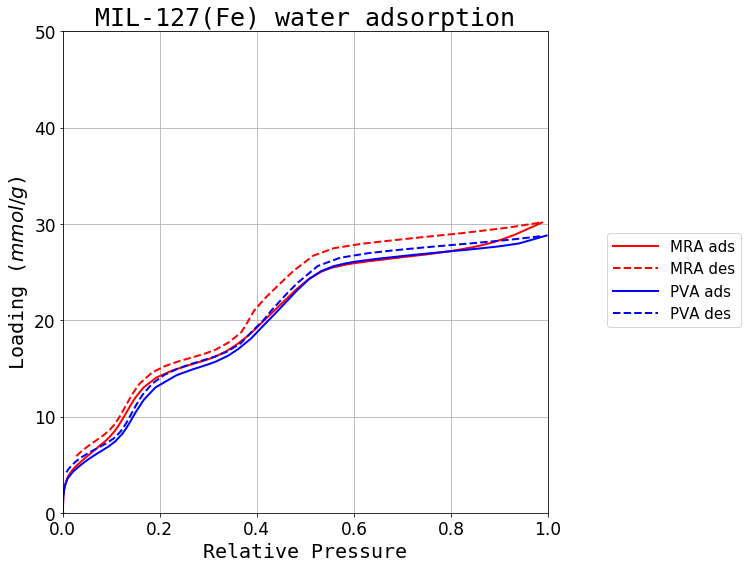
\includegraphics[width=0.45\textwidth]{water/MIL-127(Fe)-water}%
        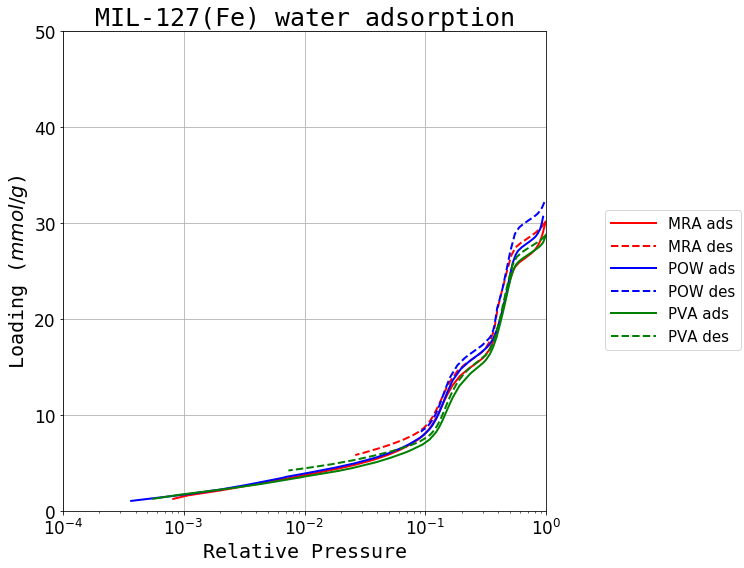
\includegraphics[width=0.45\textwidth]{water/MIL-127(Fe)-water-log}%
        \caption{}\label{shaping:fig:watermil127}%
    \end{subfigure}%
    
    \caption{Water adsorption isotherms (a) UiO-66(Zr), 
    (b) MIL-100(Fe) and (c) MIL-127(Fe). The powder samples are in light
    blue, while the \(\rho\)-alumina and poly-vinyl alcohol samples are
    in red and dark blue respectively. Logarithmic graphs of the
    isotherms are on the right for clarity of the low
    pressure region.}%
    \label{shaping:fig:wateradsorption}
\end{figure}

Two visual indicators may highlight changes in material hydrophilicity: 
the slope of the isotherm in the low relative pressure region 
(\(p/p_0 < 0.3\)) and condensation steps in the isotherm. 
Adsorption at low pressures is representative of the initial
interactions with the surface, as discussed in the previous section.
The pressure at which condensation occurs in the pores of the material, 
underlined by a sharp increase in the isotherm, depends on the 
size of the pore but also on pore environment and 
guest-guest interactions. Finally, hysteresis in the adsorption 
isotherm may also be an indication of the nature of pores.

The measured isotherms on water and methanol can be found
in \autoref{shaping:fig:wateradsorption} 
and \autoref{shaping:fig:methanoladsorption} respectively.
Initial Henry constants \gls{kH0} have been calculated for the isotherms
using the initial point method, and are displayed in
\autoref{shaping:fig:vapourkh}.

\begin{figure}[htb]
    \centering
    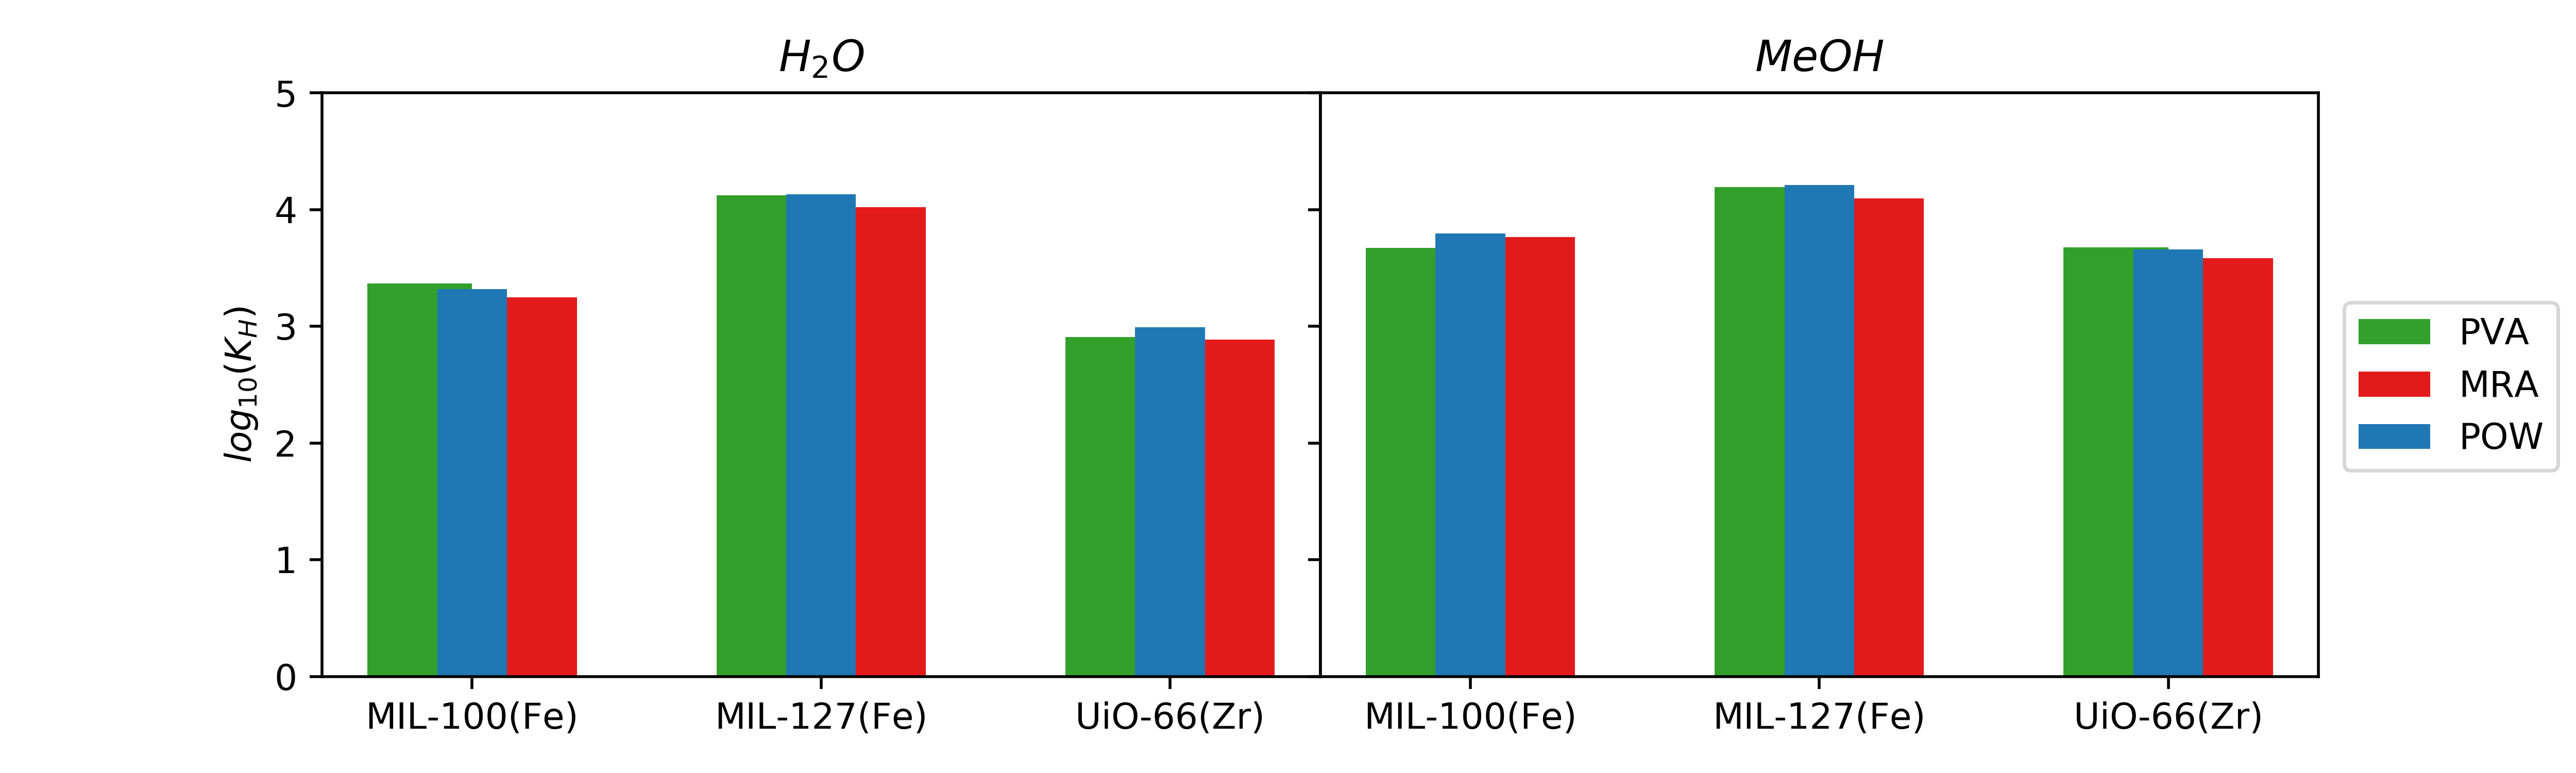
\includegraphics[width=\linewidth]{vapourkh}%
    \caption{Calculated initial Henry constant for
    the vapour adsorption isotherms 
    in \autoref{shaping:fig:wateradsorption}
    and \autoref{shaping:fig:methanoladsorption}}%
    \label{shaping:fig:vapourkh}
\end{figure}

\begin{figure}[p!]
    \centering

    \begin{subfigure}{\linewidth}
        \centering
        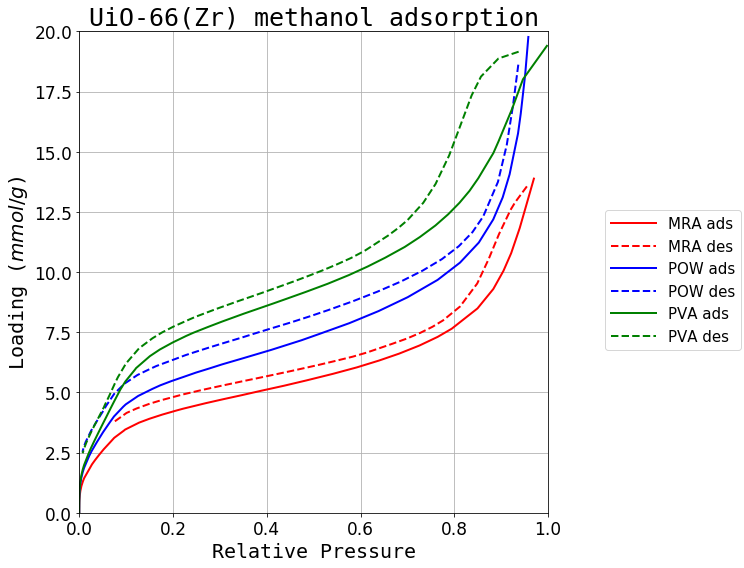
\includegraphics[width=0.45\textwidth]{methanol/UiO-66(Zr)-methanol}%
        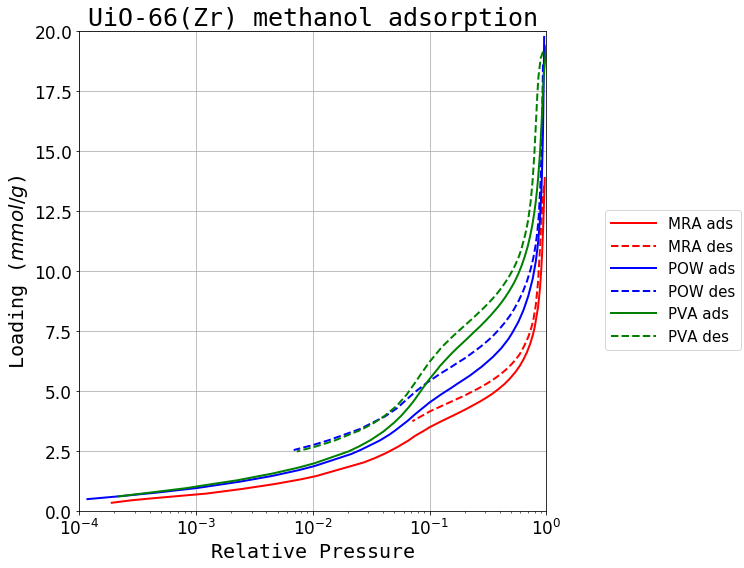
\includegraphics[width=0.45\textwidth]{methanol/UiO-66(Zr)-methanol-log}%
        \caption{}\label{shaping:fig:methanoluio66}%
    \end{subfigure}%

    \begin{subfigure}{\linewidth}
        \centering
        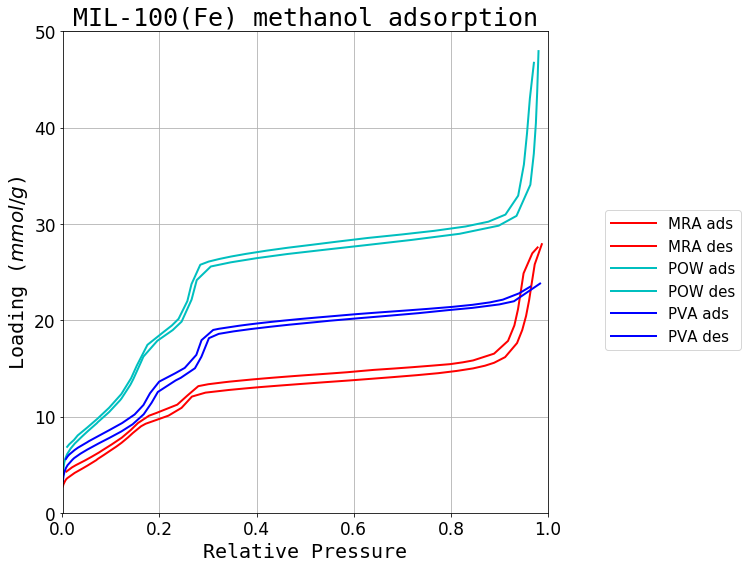
\includegraphics[width=0.45\textwidth]{methanol/MIL-100(Fe)-methanol}%
        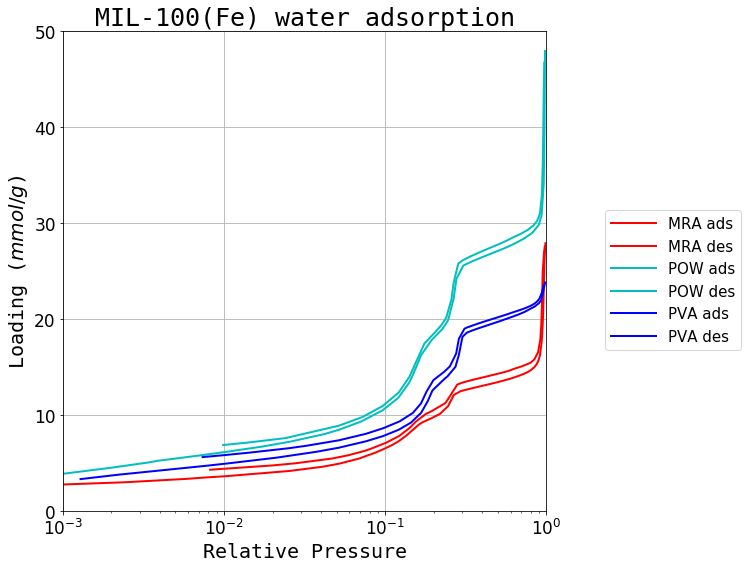
\includegraphics[width=0.45\textwidth]{methanol/MIL-100(Fe)-methanol-log}%
        \caption{}\label{shaping:fig:methanolmil100}%
    \end{subfigure}%

    \begin{subfigure}{\linewidth}
        \centering
        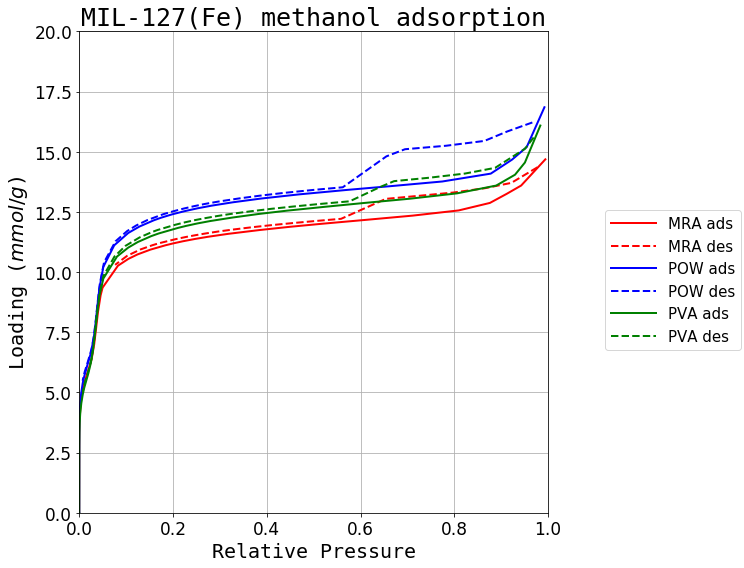
\includegraphics[width=0.45\textwidth]{methanol/MIL-127(Fe)-methanol}%
        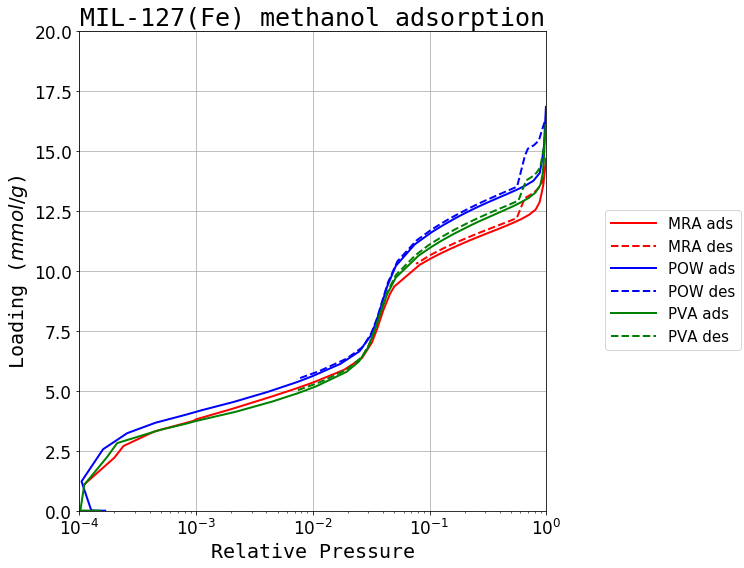
\includegraphics[width=0.45\textwidth]{methanol/MIL-127(Fe)-methanol-log}%
        \caption{}\label{shaping:fig:methanolmil127}%
    \end{subfigure}%
    
    \caption{Methanol adsorption isotherms (a) UiO-66(Zr), 
    (b) MIL-100(Fe) and (c) MIL-127(Fe). The powder samples are in light
    blue, while the \gls{MRA} and \gls{PVA} samples are in red
    and dark blue respectively. Logarithmic 
    graphs of the isotherms are on the right for clarity of the low
    pressure region.}%
    \label{shaping:fig:methanoladsorption}
\end{figure}

\subsubsection{UiO-66(Zr)}

On the parent UiO-66(Zr), the water isotherm shows a slow uptake 
at the start, indicating a hydrophobic surface, and then shows 
a small step at \(p/p_0 = 0.3\). While little is 
adsorbed on the \gls{MOF} before this step, its presence 
at a low relative humidity is indicative of intrinsic defects
in the framework~\cite{ghoshWaterAdsorptionUiO662014}.
Complete saturation takes place around \(p/p_0 = 0.9\). 
A wide hysteresis curve can be seen, which 
does not fully close, even at low pressures. Both the
saturation step and the condensation may be attributed 
to agglomeration of crystals and interparticle voids.

The methanol isotherm has the same features as the water
one, with the condensation step shifted at a much lower 
partial pressure (\(10^{-1} p/p_0\)). It is likely that
the organic component of methanol interacts with the
hydrophobic surface, thus permitting pore filling at
lower pressures. This is also evidenced through the higher
Henry constant when compared to water.

When comparing the powder and the pellet variants, the 
general shape of the isotherm remains the same with both
water and methanol. Initial interactions with the surface are also
identical, as evidenced by the overlap in the low pressure region
and through the calculated Henry constants. The isotherms 
begin to diverge after the condensation step, where the 
maximum loading evolves in the order \gls{MRA} < powder < \gls{PVA}
for both vapours. This is a surprising trend, as both pellets
have been shown to have lower capacities than the powder,
stemming from material amorphization during granulation.
The addition of hydrophilic alumina conforms to this hypothesis,
and appears to have no impact on the initial interaction with 
the surface. On the other hand, polymer-shaped particles
seem to have a higher maximum capacity than both powder and 
alumina pellets. It is unclear if this effect is due to a 
cooperative effect of hydrogen bonding with hydroxyl groups 
on the polymer chains or has another underlying cause.


\subsubsection{MIL-100(Fe)}

The methanol isotherm (\autoref{shaping:fig:methanolmil100}) on 
the same parent \gls{MOF} still shows 
two condensation steps, which have been shifted at a much
lower pressure. There is no longer any hysteresis present,
an indication that the critical pore radius for its formation
is not attained when using methanol.

When comparing the powder isotherms with their shaped counterparts,
while the general features of the isotherm remain the same, 
large shifts are seen in the capacity at different pressures.
Adsorption of \ce{H2O} proceeds in an identical fashion
on all forms until the condensation step at \(0.3~p/p^0\), where
the alumina binder variant diverges to reach a plateau about
\SI{5}{\milli\mol\per\gram} smaller than the \gls{PVA} and powder
isotherms. The shape of the hysteresis loop also changes slightly,
with a sharper slope on the adsorption branch that closes 
before \(0.5~p/p^0\). Some changes can also be seen on the methanol
adsorption isotherm, where the condensation steps are shifted 
towards lower pressures. These features are a likely sign of 
the pore filling of the alumina binder.
However, no influence is seen on the initial filling behaviour
as the Henry's constant confirms that low pressure 
interactions do not change. 

In terms of the pore volume, the \gls{MRA} isotherms 
show the most drastic loss, consistent with the values 
obtained with nitrogen at \SI{77}{\kelvin} and room temperature
calorimetry experiments. On the other hand, polymer pellets differ 
between the two vapours, with almost no capacity loss on water 
and a large drop with methanol. A possible explanation is 
pore occlusion, with the small cage windows being covered by 
polymer chains. As the size of the water molecule is smaller 
than methanol, more porosity is accessible through this probe.

It is also interesting to note that the
``gating'' effect seen with butane adsorption on the \gls{PVA} pellets
in the original study~\cite{chanutObservingEffectsShaping2016}
is not seen in the measured vapour isotherms, likely due to the 
small kinetic radius of both probes.

\subsubsection{MIL-127(Fe)}

On the last \gls{MOF} powder, the water isotherm 
(\autoref{shaping:fig:watermil127}) shows a hydrophilic
surface, with a highest initial slope out of the three 
materials studied. The isotherm has two condensation steps,
a low relative humidity one at \(0.15~p/p_0\), which corresponds
to the filling of the hydrophilic pore, and a condensation 
step situated at \(0.5~p/p_0\) inside the more hydrophobic micropore.
No hysteresis is observed.

As a striking difference from water behaviour, methanol adsorption
leads to completely filled pores at below \(0.15\) relative 
pressure. By examining the logarithmic isotherms in 
\autoref{shaping:fig:methanolmil127} a steep slope at low
pressures is evident. It is likely that the larger size of the
methanol molecule is much more affected by confinement in 
the hydrophilic pore, and leads to sudden micropore filling.
The same effect, combined with the increased affinity for the 
organic part of the probe is likely responsible for shifting the 
secondary condensation step at lower pressures.

The similarities between the both variants of shaped pellets 
and the original powder confirms the previously observed 
suitability of this \gls{MOF} towards the shaping process. The isotherms
overlap almost fully, with a slight difference in maximum uptake
in the order of powder > \gls{PVA} > alumina. The binder has not affected
the interaction with the guest, as evidenced by the near-identical
initial Henry constant.